\documentclass[10pt]{article}
\usepackage{amssymb,amsmath,amsthm,longtable}
\usepackage{latexsym}
\usepackage{placeins}
\usepackage{graphicx}
\usepackage{caption}
\usepackage{textcomp}
\captionsetup{width=5.75in}
\usepackage[top=1in, bottom=1in, left=1in, right=1in]{geometry}

\numberwithin{equation}{section}
\usepackage{amsfonts}
\usepackage{upgreek}
\usepackage{bm}
\usepackage{dsfont}
\usepackage{dcolumn}
\usepackage{epsfig}
\usepackage{graphics}
\usepackage{subfigure}

% begin equation, itemize, etc.

\def\be{\begin{equation}}
\def\ee{\end{equation}}
\def\bi{\begin{itemize}}
\def\ei{\end{itemize}}
\def\ben{\begin{enumerate}}
\def\een{\end{enumerate}}
\def\i{\item{}}
\newcommand{\bs}[1]{\boldsymbol{#1}}
\newcommand{\mb}[1]{\mathbf{#1}}
\renewcommand{\vec}[1]{\mathbf{#1}}
\newcommand{\vecs}[1]{\bs{#1}}
\newcommand{\unit}[1]{\hat{\vec{#1}}}
\def\d{{\rm{d}}}

\begin{document}

%%%%%%%%%%%%%%%%%%%%%%%%%%%%%%%%%%%%%%%%%%%%%%%%%%%%%%%%%%%%%%%%%%%%%%
\title{What should I know how to do?}
\maketitle

%\tableofcontents

%%%%%%%%%%%%%%%%%%%%%%%%%%%%%%%%%%%%%%%%%%%%%%%%%%%%%%%%%%%%%%%%%%%%%%
\section{Lagrangian mechanics (\S1-5)}

\ben

\i Write down the Lagrangian for a simple system in terms of 
generalized coordinates.

Example:
%
\be
L(x,\dot x, t) = \frac{1}{2}m\dot x^2 - \frac{1}{2}kx^2
\ee
%
More generally:
%
\be
L(q,\dot q, t)= T-U
= \frac{1}{2}\sum_{i,k}a_{ik}(q) \dot q_i\dot q_k - U(q_1,q_2,\cdots, q_n, t)
\ee

\i Distinguish generalized coordinates from Cartesian coordinates.

Example: Double pendulum
%
\begin{figure}[htbp!]
\begin{center}
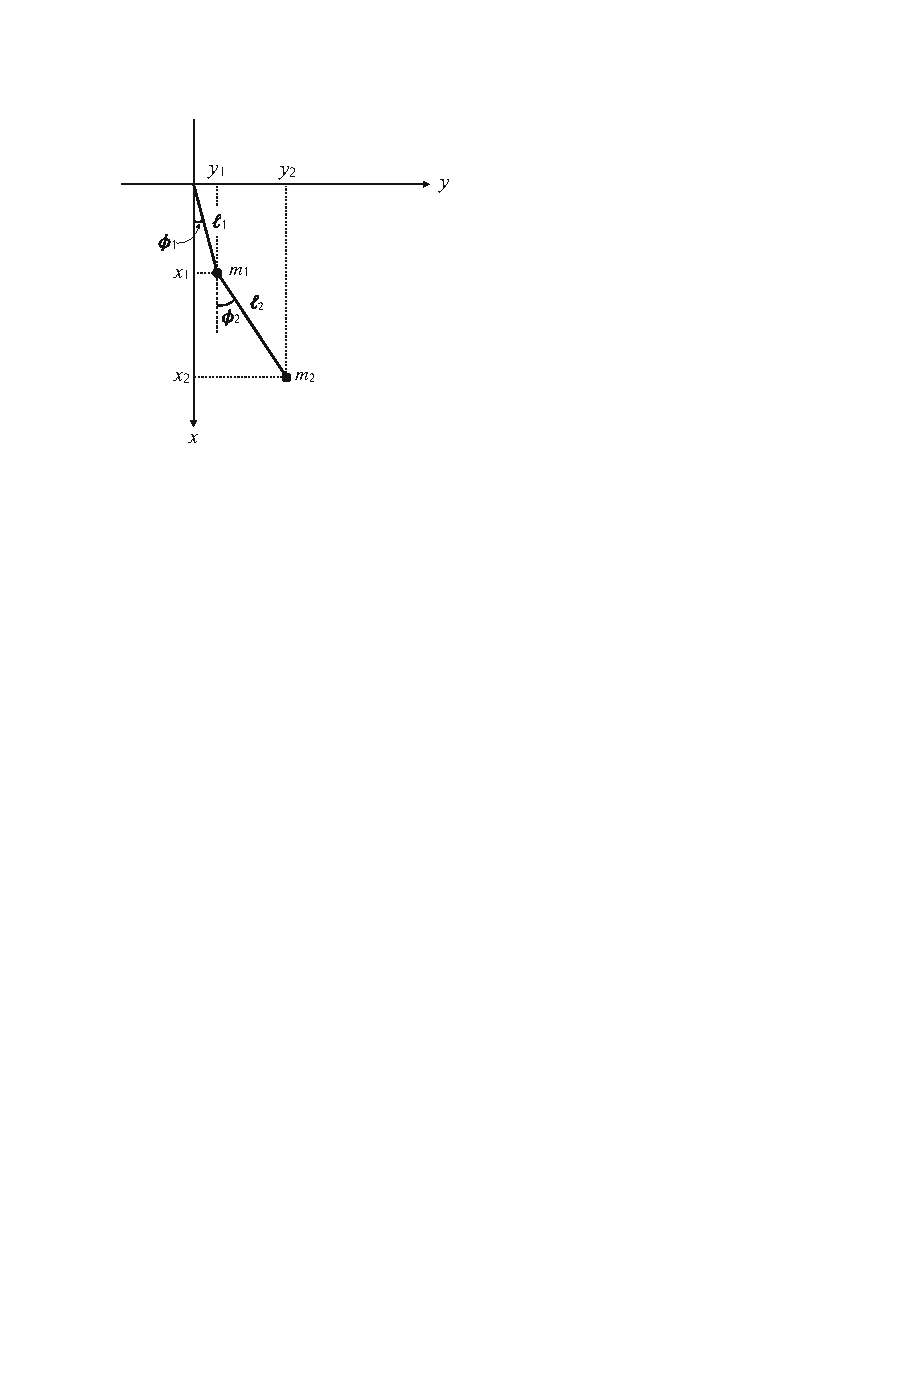
\includegraphics[width=0.4\textwidth]{img/double_pendulum}
\caption{}
\label{f:doublependulum}
\end{center}
\end{figure}
%

Use the two angles $\phi_1$, $\phi_2$ for the generalized coordinates
$q_1$, $q_2$, as opposed to the Cartesian coordinates $(x_1,y_1)$ and
$(x_2,y_2)$, which are subject to constraints imposed by the pendulum rods.

\i Write down Lagrange's equations.

\be
\frac{d}{dt}\left(\frac{\partial L}{\partial \dot q_i}\right)
= \frac{\partial L}{\partial q_i}\,,
\qquad i=1,2,\cdots, n
\ee
%
This is of the form
%
\be
\frac{dp_i}{dt} = F_i
\qquad i=1,2,\cdots, n
\ee
%
where $p_i\equiv \partial L/\partial \dot q_i$ and $F_i = -\partial
U/\partial q_i$, for the case where the kinetic energy 
$T$ does not depend explicitly on $q$.

\i Define the action in terms of the Lagrangian, and derive Lagrange's
equations starting from the action.

Action:
%
\be
S[q] \equiv \int_{t_1}^{t_2} dt\> L(q,\dot q, t) 
\ee
%
Lagrange's equations are obtained by setting $\delta S=0$ for
variations $\delta q$ that vanish at the end points $t_1$ and $t_2$.  

The following derivation is for a single degree of freedom.  For
multiple degrees of freedom, we should vary each $q_i(t)$,
$i=1,2,\cdots, n$ independently.

Derivation:
%
\be
\delta S 
= \int_{t_1}^{t_2} dt\> \left[
\frac{\partial L}{\partial q}\delta q +
\frac{\partial L}{\partial \dot q}\delta \dot q\right]
\ee
%
Integrate the second term by parts using 
\be
\delta \dot q \equiv 
\delta\left(\frac{d q}{d t}\right) 
= \frac{d}{dt}\delta q
\ee
%
obtaining
%
\be
\delta S 
= \int_{t_1}^{t_2} dt\> \left[
\frac{\partial L}{\partial q}
-\frac{d}{dt}\left(\frac{\partial L}{\partial \dot q}\right)\right] \delta q
+ \frac{\partial L}{\partial\dot q}\delta q\bigg|_{t_2}
- \frac{\partial L}{\partial\dot q}\delta q\bigg|_{t_1}
\ee
%
The last two terms vanish given the condition that the variations
$\delta q_i$ vanish at $t_1$ and $t_2$.  Since $\delta q$ is
arbitrary, setting $\delta S=0$ is equivalent to the integrand
vanishing:
%
\be
\frac{\partial L}{\partial q}-\frac{d}{dt}\left(\frac{\partial L}{\partial \dot q}\right) = 0
\ee

\i Show that Lagrange's equations are unchanged if one adds a
total time derivative $\d f(q,t)/\d t$ to $L$.

Define
%
\be
\bar{L}(q,\dot q,t) \equiv L(q,\dot q, t) + \frac{df(q,t)}{dt}
\ee
%
Then
%
\be
\bar{S}[q] \equiv \int_{t_1}^{t_2} dt\> \bar{L}(q,\dot q, t) 
= S[q] + f(q,t)\big|_{t_2} - f(q,t)\big|_{t_1}
\ee
%
From this we see that $\delta \bar{S}=\delta S$, since $\delta
q|_{t_1}=0$ and $\delta q|_{t_2}=0$.  So the EOMs from $L$ and
$\bar{L}\equiv L + df(q,t)/dt$ are the same.

Note: one can obtain the same result by working directly with
Lagrange's equations for $L$ and $\bar L$.

\i Include both holonomic and non-holonomic constraint forces 
in the Lagrangian formalism by introducing Lagrange multipliers.

(i) Holonomic constraints are relationships between the generalized
coordinates and possibly time
%
\be
\varphi_\alpha(q,t)=0\,,
\qquad \alpha=1,2,\cdots,m
\label{e:holonomic}
\ee
%
where $\alpha$ labels the different constraints.
Such constraints can be included in the Lagrangian formalism
by augmenting the Lagrangian as follows:
%
\be
L(q,\dot q, t) 
\quad \rightarrow\quad
L(q,\dot q, t) + \sum_\alpha \lambda_\alpha(t) \varphi_\alpha(q,t)
\ee
%
where the $\lambda_\alpha(t)$ are so-called Lagrange multipliers.  The
modified equations of motions are then
%
\be
\frac{d}{dt}\left(\frac{\partial L}{\partial \dot q_i}\right)
= \frac{\partial L}{\partial q_i} + \sum_\alpha
\lambda_\alpha\frac{\partial\varphi_\alpha}{\partial q_i}\,,
\qquad i = 1,2,\cdots, n
\ee
%
Together with the constraint equations \eqref{e:holonomic}, these are $n+m$ 
equations for the $n+m$ unknowns $q_i$ and $\lambda_\alpha$.
Note that the generalized constraint force
$\sum_\alpha \lambda_\alpha (\partial \varphi_\alpha/\partial q_i)$ is
orthogonal to the constraint surface \eqref{e:holonomic}.

(ii) Non-holonomic constraints are relationships between the coordinate
differentials 
%
\be
\sum_i c_{\alpha i}\,\delta q_i = 0\,,
\qquad \alpha = 1,2,\cdots, m
\label{e:nonholonomic}
\ee
%
that cannot be integrated to yield relations between just the
generalized coordinates.
Such constraints can be included in the Lagrangian formalism 
at the level of the variation of the action.
The modified equations of motion are
%
\be
\frac{d}{dt}\left(\frac{\partial L}{\partial \dot q_i}\right)
= \frac{\partial L}{\partial q_i} +
\sum_\alpha \lambda_\alpha c_{\alpha i}\,,
\qquad i=1,2,\cdots, n
\ee
%
where $\lambda_\alpha(t)$ are Lagrange multipliers.
Together with \eqref{e:nonholonomic}, these are $n+m$ equations 
for the $n+m$ unknowns $q_i$ and $\lambda_\alpha$.

Examples of non-holonomic constraints include dissipative 
forces like friction, and the reaction force for a 
sphere that rolls without slipping or pivoting on a 
horizontal surface:
%
\be
\vec V - \vecs\Omega\times(a\unit n) = 0
\ee
%
where $\vec V$ is the velocity of the COM of the sphere
of radius $a$, $\vecs\Omega$ is the angular velocity vector,
and $\unit{n}$ is a unit vector normal to the surface.

\i Define and give examples of a {\em closed system}, 
{\em constant external field}, and {\em uniform field}.

{\em Closed system:}

The potential $U$ is a function of only the relative position vectors
$\vec r_1-\vec r_2$, etc. 

{\em Constant external field:}
\be
U \equiv U(\vec r_1, \vec r_2, \cdots, \vec r_N)
\ee
has no explicit time dependence

{\em Uniform field:}
\be
U = -\sum_a \vec F_a\cdot \vec r_a
\ee
where $\vec F_a$ is independent of $\vec r_1$, $\vec r_2$, etc., so that 
\be
-\frac{\partial U}{\partial\vec r_a}= \vec F_a
\quad{\rm has\ no\ position\ dependence}
\ee

\een

%%%%%%%%%%%%%%%%%%%%%%%%%%%%%%%%%%%%%%%%%%%%%%%%%%%%%%
\section{Non-inertial reference frames (\S39)}

\ben

\i Write down the relationship between velocity vectors 
in inertial and non-inertial reference frames.

See Figure~\ref{f:noninertial}:
%
\be
\vec v_0 
\equiv \dot{\vec r}_0
= \vec V + \vec v + \vecs\Omega\times\vec r
\ee
%
where $\vec V\equiv\dot{\vec R}$ is the velocity of the origin $O$
wrt to the inertial frame, and 
$\vec v$ is the velocity of $m$ wrt the non-inertial frame.

%
\begin{figure}[htbp!]
\begin{center}
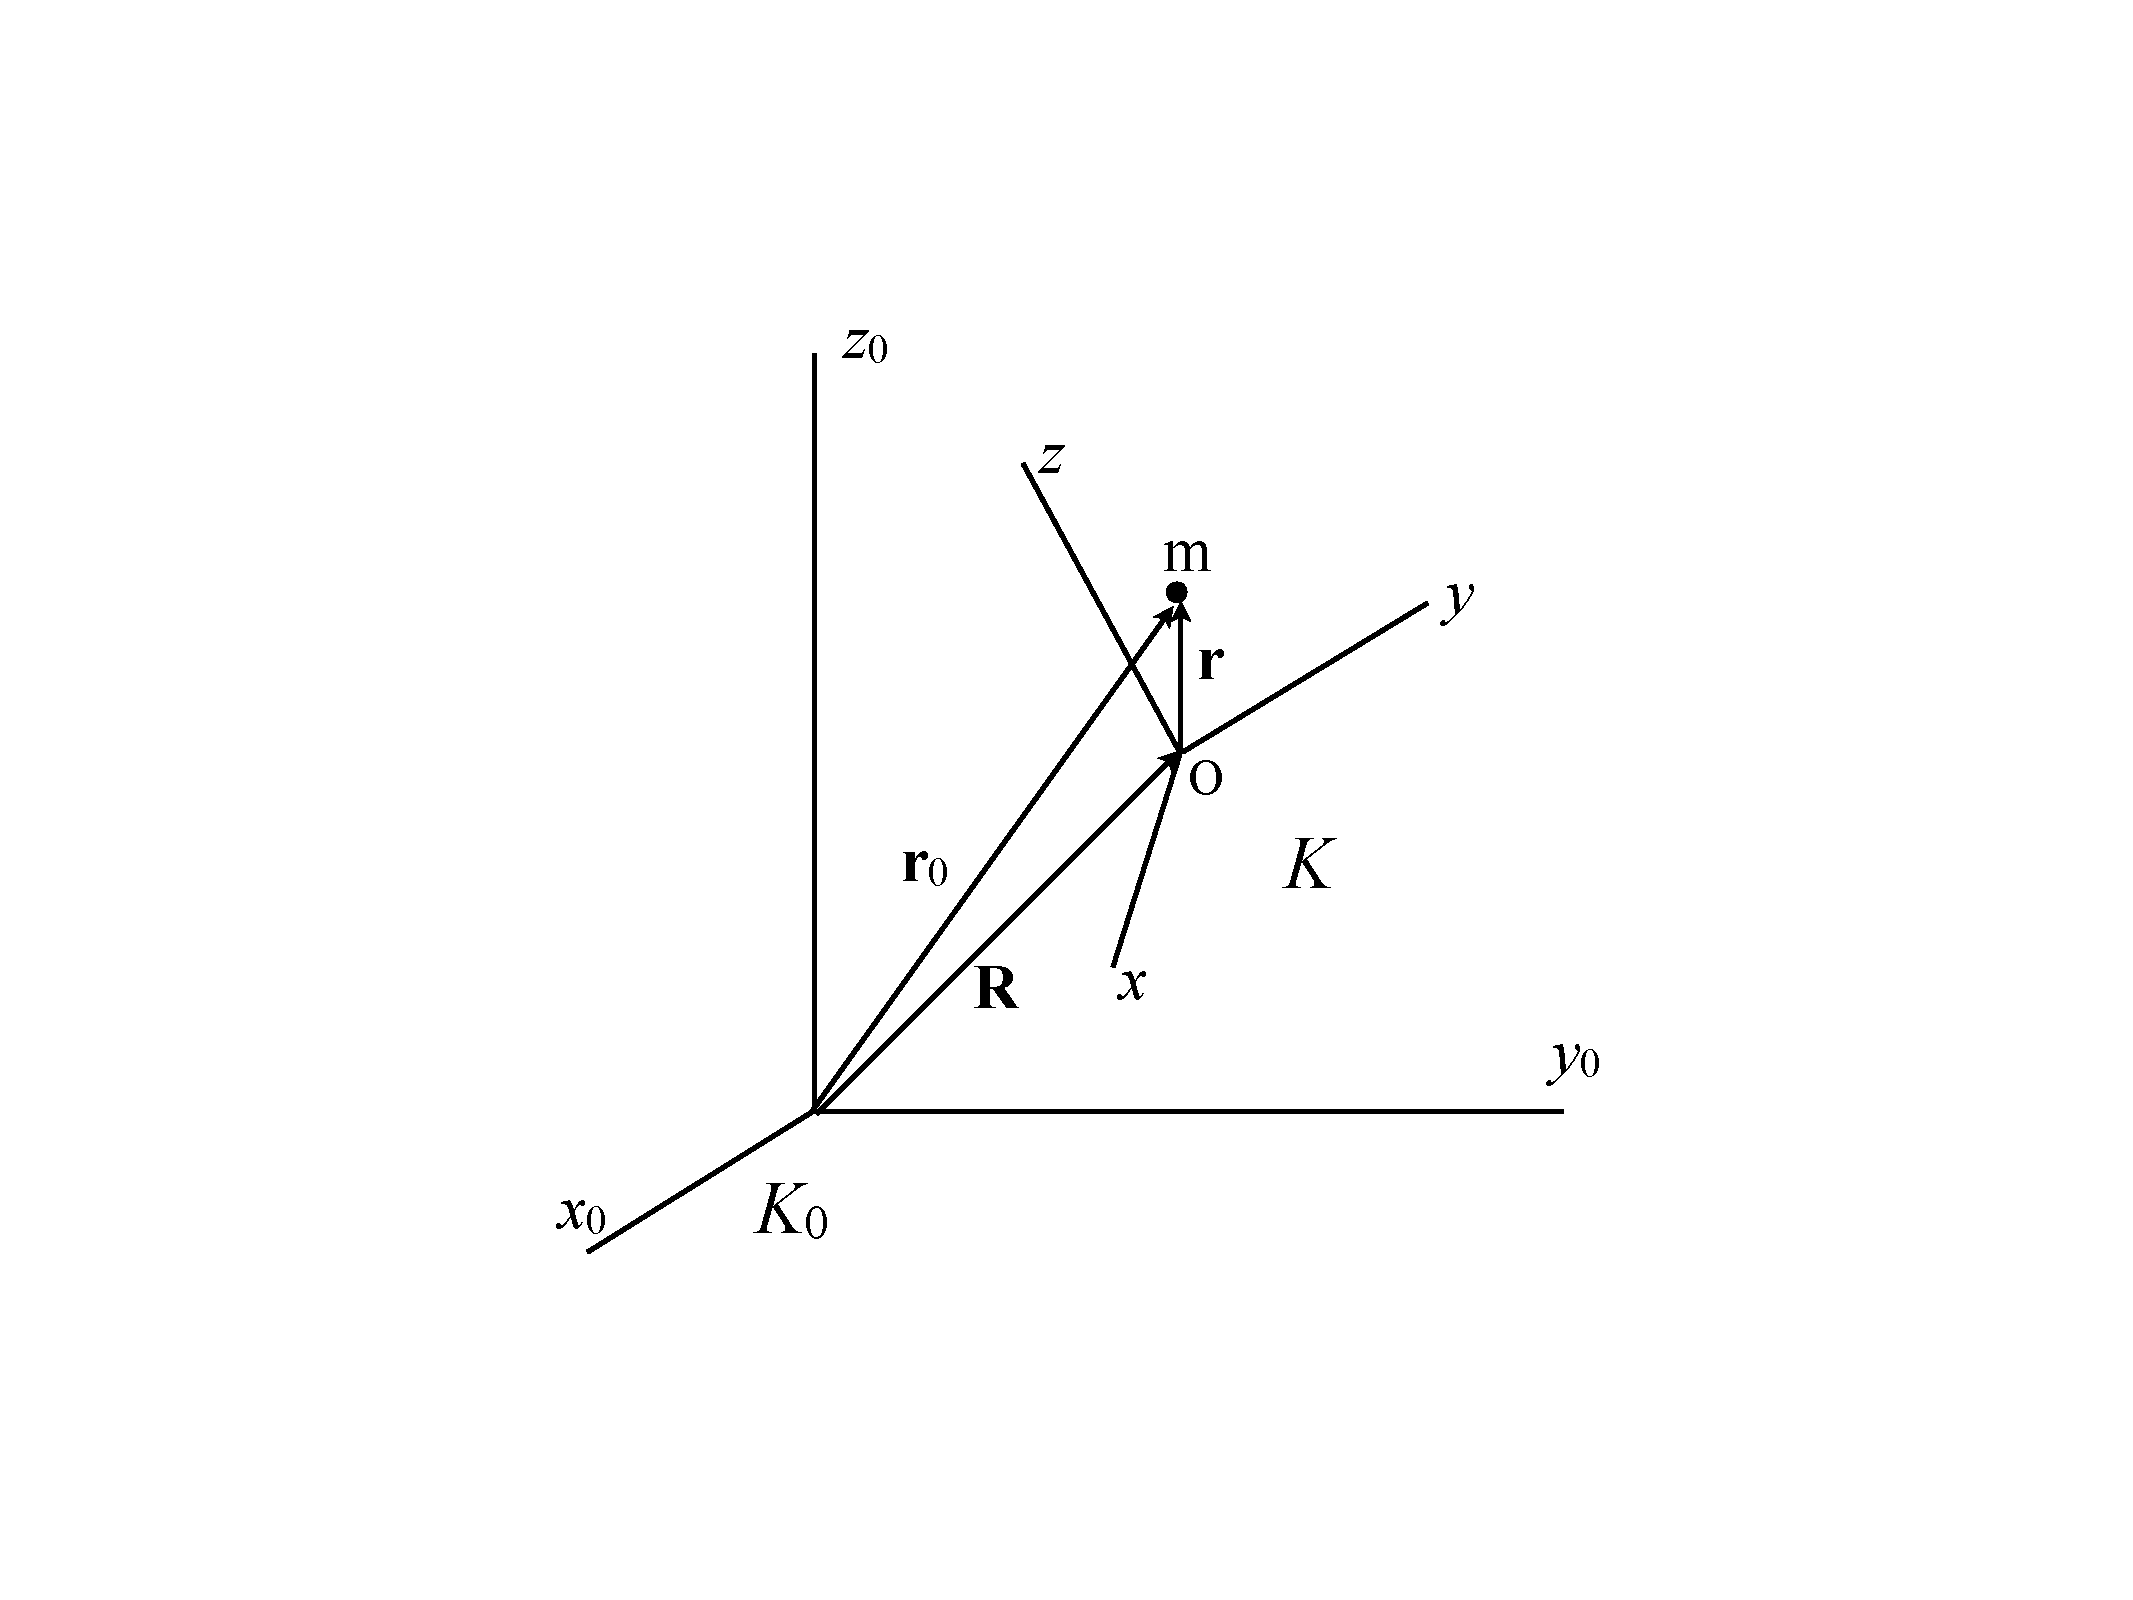
\includegraphics[width=0.4\textwidth]{img/noninertial}
\caption{}
\label{f:noninertial}
\end{center}
\end{figure}
%

\i Distinguish non-inertial reference frames associated
with translational and rotational motion.

\i Give examples of the Coriolis, centrifugal, translational 
acceleration, and rotational acceleration fictitious force terms.

\i Explain the physical significance of Foucault's pendulum.

\een

%%%%%%%%%%%%%%%%%%%%%%%%%%%%%%%%%%%%%%%%%%%%%%%%%%%%%%
\section{Hamiltonian mechanics (\S40)}

\ben

\i Write down the Hamiltonian $H(p,q,t)$ for a simple 
system starting from a Lagrangian $L(q,\dot q,t)$.

\i Write down Hamilton's equations for $p_i$ and $q_i$.

\i Explain the fundamental difference between Hamilton's 
equations and Lagrange's equations.

\i Show the equivalence of Hamilton's equations and Lagrange's equation
for simple systems.

\een

%%%%%%%%%%%%%%%%%%%%%%%%%%%%%%%%%%%%%%%%%%%%%%%%%%%%%%%%%%%%%%%%%%%%%%
\section{Conservation laws (\S6-10)}

\ben

\i Show how conservation of energy, momentum, and angular 
momentum are connected to time translation, space translation, 
and rotational symmetry, respectively.

\i Write down the general expression for the 
energy function $E$.

\i Explain what it means for a function to be a homogeneous
function of degree $k$.

\i Write down the expression for the generalized momentum $p_i$.

\i Write down the expression for the center of mass (COM) of
a system of particles.

\i Write down the virial theorem for a system whose motion 
takes place in a finite region of space and whose potential 
energy is a homogoneous function of degree $k$ in the coordinates.
 
\een

%%%%%%%%%%%%%%%%%%%%%%%%%%%%%%%%%%%%%%%%%%%%%%%%%%%%%%%%%%%%%%%%%%%%%%
\section{Central force motion (\S11, 13-15)}

\ben

\i Write down an integral expression for $t$ for 1-d motion
in a fixed external field $U(x)$.

\i Determine the allowed values of the energy and turning
points for 1-d motion in a fixed external field.

\i Transform the problem of two interacting particles into 
an effective one-body problem by working in the COM frame.

\i Write down the kinetic energy of two interacting particles
in the COM frame in terms of the time derivative of the relative
position vector $\vec r\equiv \vec r_1-\vec r_2$.

\i Write down expressions for the reduced mass and total mass
of the system for the effective one-body problem.

\i Show that both energy and angular momentum are 
conserved for a central potential.

\i Write down an expression for the effective potential 
$U_{\rm eff}(r)$ in terms of $U(r)$ and $\ell$.

\i Plot the effective potential for some simple central force
potentials.

\i From the graph of the effective potential, determine the 
different types of allowed motion.

\i Write down integral expressions for $t$ and $\phi$ in terms
of $r$ for a general central potential.

\i Evaluate these two integrals for Kepler's problem, using
appropriate trig substitutions.

\i Derive the relationship between $E$, $\ell$, $a$, $b$,
$e$, and $p$ for an ellipse.

\i State the only two central potentials that have closed 
bound orbits.

\i State and derive Kepler's three laws of planetary motion.

\i Explain the difference in $E$ and $e$ for elliptical, parabolic,
and hyperbolic motion.

\een

%%%%%%%%%%%%%%%%%%%%%%%%%%%%%%%%%%%%%%%%%%%%%
\section{Collisions and scattering (\S16-20)}

\ben

\i Draw diagrams relating velocities in the lab and COM frames for 
the disintegration of a single particle.

\i Draw diagrams relating the momenta in the lab and COM frames 
for an elastic collision of two particles ($m_2$ initially at 
rest in the lab frame).

\i Explain what information can and cannot be provided for an 
elastic collison of two particles, just using conservation of 
momentum and conservation of kinetic energy.

\i Derive formulas relating the scattering angles $\chi$,
$\theta_1$, $\theta_2$ in the COM and lab frames.

\i Draw diagrams showing how the scattering angle $\chi$ is 
related to the angle of closest approach $\phi_0$.

\i Relate the impact parameter $\rho$ and initial velocity 
$v_\infty$ to the energy $E$ and angular momentum $\ell$.

\i Integrate (18.4) for $\phi_0$ for simple potentials---e.g., 
$U(r) = \alpha/r$ for Rutherford scattering.

\i Write down expressions for 
${\rm d}\sigma$ in terms of ${\rm d}\rho$, ${\rm d}\chi$, ${\rm d}\theta_1$, 
${\rm d}\theta_2$, or ${\rm d}\Omega$, ${\rm d}\Omega_1$, ${\rm d}\Omega_2$.

\i Explain how one can obtain an expression for small-angle 
scattering starting from (18.4) for $\phi_0$.

\een

%%%%%%%%%%%%%%%%%%%%%%%%%%%%%%%%%%%%%%%%%%%%%
\section{Small oscillations (\S21-23)}

\ben
\i Explain what stable equilibrium means in terms of the 
potential energy $U(q)$.

\i Calculate the frequency for small oscillations about 
a position of stable equilibrium.

\i Solve the equations of motion for both free and 
forced oscillation in one dimension, noting the difference
between the {\em general solution} of the 
homogeneous equation and a {\em particular integral} 
of the inhomogeneous equation.
 
\i Calculate the eigenfrequencies / eigenvectors for
small oscillations of systems with more than one DOF.

\een

%%%%%%%%%%%%%%%%%%%%%%%%%%%%%%%%%%%%%%%%%%%%%
\section{Rigid body motion (\S31-36, 38)}

\ben
\i Write down an expression for the components  $I_{ik}$
of the inertia tensor as a sum over discrete mass points 
or as an integral over the volume of the body.

\i Obtain or identify the {\em principal axes of
inertia} for various rigid bodies.

\i Calculate the 
{\em principal moments of inertia} for various rigid bodies.

\i Calculate the kinetic energy of a rigid body in terms of
its COM motion and rotational kinetic energy.

\i Write down an expression for the angular 
momentum vector $\vec M$ in terms $I_{ik}$ and ${\Omega}_i$.

\i Write down the equations of motion for a rigid body with 
respect to an inertial frame.

\i Derive Euler's equations for rigid body motion (equations 
of motion in the body frame).

\i Draw a diagram showing the definition of the Euler angles
$(\phi,\theta,\psi)$.

\i Calculate the components of $\vecs{\Omega}$ wrt body 
frame in terms of the Euler angles and their time derivatives.

\i Solve for the reaction forces for rigid bodies in static equilibrium.
\een
\end{document}
